%%%%%%%%%%%%%%%%%%%%%%% file template.tex %%%%%%%%%%%%%%%%%%%%%%%%%
%
% This is a template file for Web of Conferences Journal
%
% Copy it to a new file with a new name and use it as the basis
% for your article
%
%%%%%%%%%%%%%%%%%%%%%%%%%% EDP Science %%%%%%%%%%%%%%%%%%%%%%%%%%%%
%
%%%\documentclass[option]{webofc}
%%% "twocolumn" for typesetting an article in two columns format (default one column)
%
\documentclass{webofc}
\usepackage[varg]{txfonts}   % Web of Conferences font
%
% Put here some packages required or/and some personal commands

\usepackage{xspace}
\usepackage{tabularx}

\newcommand{\pd}{protoDUNE\xspace}
\newcommand{\filesize}{8\,GB\xspace}


%
%
\begin{document}
%
\title{The Prompt Processing System and Data Quality Monitoring in the \pd-SP experiment}
%
%%%\subtitle{Do you have a subtitle?\\ If so, write it here}
\author{ 
\lastname{Maxim Potekhin}\inst{1}\fnsep\thanks{\email{potekhin@bnl.gov}} \it{on behalf of the DUNE Collaboration}
}

\institute{Brookhaven National Laboratory, Upton, NY11973, USA}



\abstract{%
The DUNE Collaboration is conducting an experimental program named ''protoDUNE''
which includes a beam test of two large-scale  prototypes of the Liquid Argon Time
Projection Chamber located at CERN. We present the status of prompt processing
and data quality monitoring systems deployed for the single-phase version of the detector.

}
%
\maketitle
%
\section{Introduction}
\label{sec:intro}
The \pd-SP experiment is designed to study a large-scale prototype of the single-phase version of
the Liquid Argon Time Projection Chamber (LArTPC) which will eventually become one of
the principal elements of the DUNE apparatus to be constructed at the Sanford Underground
Research Facility \cite{cdrVol1, cdrVol4}. The prototype (CERN designation NP04) is located
in the CERN North Experimental Hall and tested utilizing a dedicated beam line from the CERN SPS
accelerator complex. The run plan also includes a large number of cosmic ray triggers.
Commisioning of the detector took place in September of 2018.
%The layout of the experimental area is shown in Fig.\,\ref{fig:np02np04}, with the single-phase
%detector seen as a cubic structure (the cryostat) on the right-hand side of the diagram. 

\begin{figure}[tb]
\centering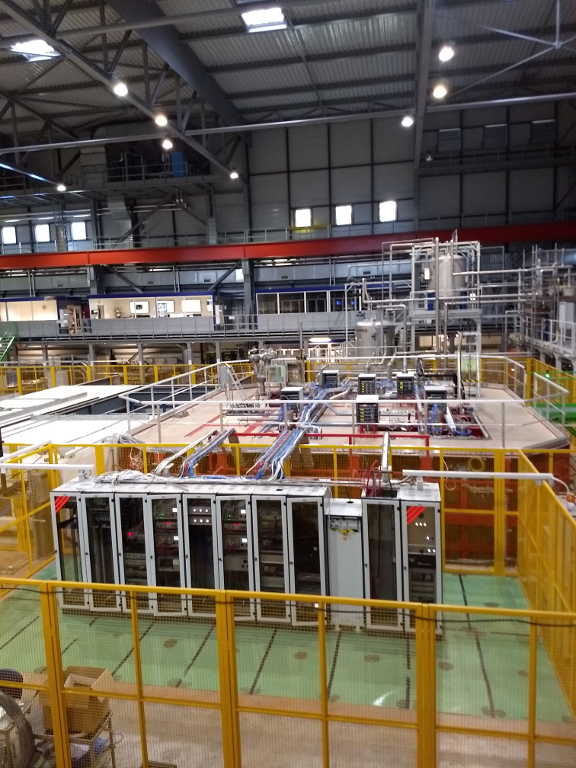
\includegraphics[width=0.7\textwidth]{figures/np04_photo_2018_v1.png}
\caption{\label{fig:np04_photo}
View of the top of the \pd-SP apparatus.
The direction of the particle beam is from left to right.
Readout systems are visible on top of the detector, with DAQ racks in front.
}
\end{figure}


In order to provide the cosmic ray triggering capability a large array of scintillation
counters is installed outside of the cryostat. A number of beam instrumentation devices
are used to feed the  trigger logic and to characterize the beam. Fig.\ref{fig:np04_photo}
shows the view of the top of the \pd-SP apparatus and a part of its readout hardware.
% Located in the vicinity of the detectors are enclosures for the online computing infrastructure
%(including Data Acquisition, Online Buffer etc) shown schematically as yellow blocks in the upper-right
%portion of  the diagram.
There is a dedicated 20 Gb/s network connection from the experiment to the CERN central storage facilities.

The \pd-SP Data Acquisition is equipped with a capable Online Monitoring System which receives data via
the network and does processing in real time. However, certain types of processing e.g.\,application of
digital filtering to the TPC channels, counting hit candidates etc which belong to the
category of Data Quality Monitoring (DQM) require more resources than are available within
the DAQ footprint, and include jobs that take substantially longer time than processes run in the
Online Monitor. That could present a resource and data management problem for the DAQ.
The Online Monitor is a real time system
and not well suited for long term preservation and cataloging of the data produced, such as plots,
histograms, tables etc as this would substantially complicate the system.

A separate consideration is the necessity to insulate DAQ from
potential disruptions due to frequent software updates of the DQM software dictated by
the dynamic nature of the test beam experiment. 
For these reasons a separate ``\pd Prompt Processing System'' (abbreviated as \textbf{p3s}) was put
in place \cite{eps} with the following characteristics:
\begin{itemize} 

\item turnaround time on the scale of minutes (and in some cases tens of minutes)

\item lower bandwidth as compared to the Online Monitor (i.e. a small fraction of events is processed,
but in more detail)

\item extensive and scalable computing resources provided on the CERN batch facility

\item reading data from files committed to CERN central storage, with no direct coupling to the DAQ system

\item flexibility in introducing, modifying and configuring software without any risk of disruption of
critical DAQ functionality

\item substantial storage and browsing capability allowing the users to access and study
the DQM results in an efficient manner

\end{itemize}

%\begin{figure}[tb]
%\centering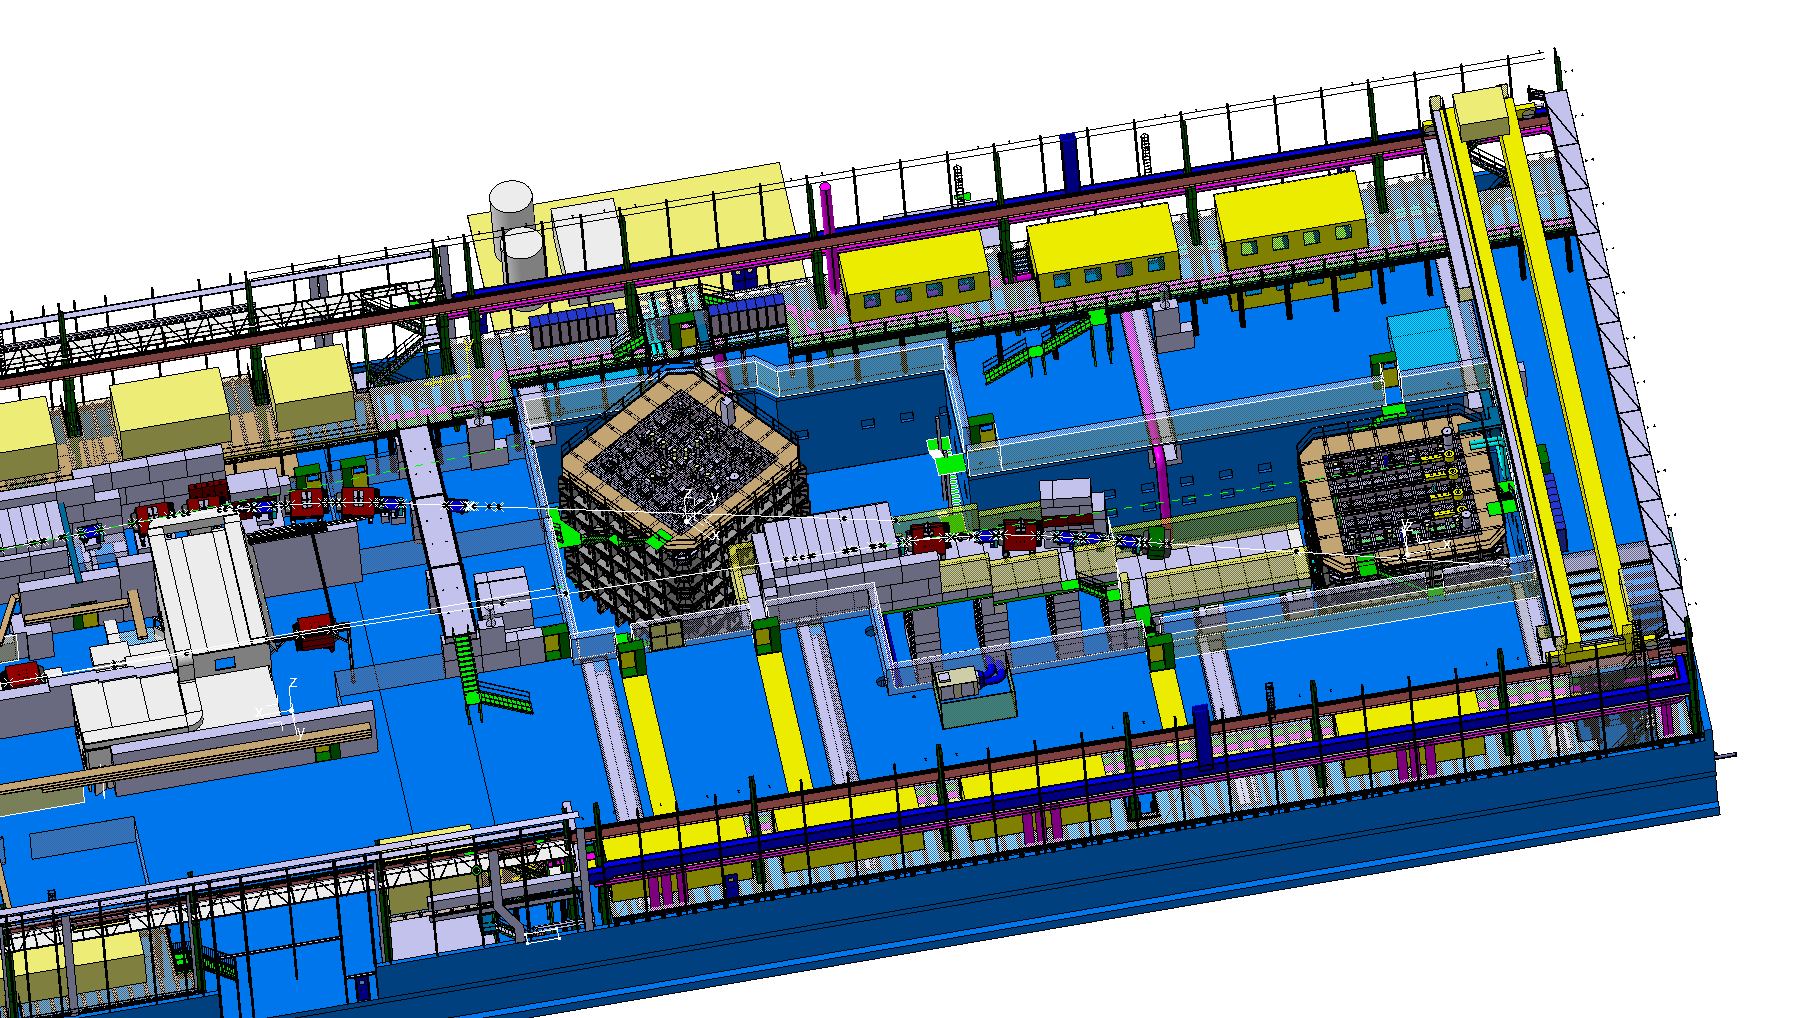
\includegraphics[width=1.0\textwidth]{figures/np02np04.png}
%\caption{\label{fig:np02np04}Diagram of the layout of the CERN north area with
 % location of the protoDUNE dual phase detector (center) and the single
  %phase detector (right). The direction of the particle beam is from left to right.}
%\end{figure}

\section{The protoDUNE-SP Data}
\subsection{Raw Data Parameters}
\label{sec:np04_data_rate}

The detector features the ``cold electronics'' design in which the amplifiers and digitizers
are placed within the cryostat and operate at cryogenic temperatures. There are
``Warm Interface Boards'' located outside of the cryostat which concentrate data
and transmit it to the DAQ systems via an optic fiber.
% Digital signals are fed to the Warm Interface Boards located outside of the cryostat on its top surface and then
% transmitted to the Data Acquisition System via a fiber optic line.
There are 15,360 TPC channels read out at the 2\,MHz digitization frequency. There is also
a Photon Detector integrated in the TPC internal structure, but the amount of data
produced by this subsystem is substantially smalled than that of the TPC.
The size of the data read out from the detector in a single trigger cycle is approximately 230\,MB. At the nominal
trigger rate and lossless compression applied in the DAQ instantaneous data rate is about
1.5\,GB/s, and the sustained data rate to disk is 300\,MB/s.

\subsection{Data Flow and Distribution}
Principal elements of data transmission and storage in \pd are illustrated in Fig.\,\ref{fig:dataflow}.
Once the raw data are captured by the Data Acquisition System and written to the Online Buffer
located in the vicinity of the detector in the experimental hall  they are picked up by an instance of
the \textit{Fermi FTS} data handling system \cite{sam,fts} which manages the transfer to EOS \cite{castoreos}
(the CERN distributed disk storage system).

EOS serves as the principal staging area  \cite{eos_role} from which the data get copied to tape
storage at CERN (``CASTOR'')  and are also transmitted to FNAL for replication, distribution and
offline processing by a separate instance of \textit{Fermi FTS}.
Importantly, EOS also serves to stage the input data for the prompt processing system and to
store and preserve  the various data products produced by DQM jobs. This design
ensures a large degree of independence of prompt processing and DQM from the DAQ and vice versa
(which is desirable),
but it also introduces a latency due to the way data transfer from the Online Buffer operates. This latency
is on the scale of a few minutes and is considered acceptable in the context of DQM.

\begin{figure}[tb]
\centering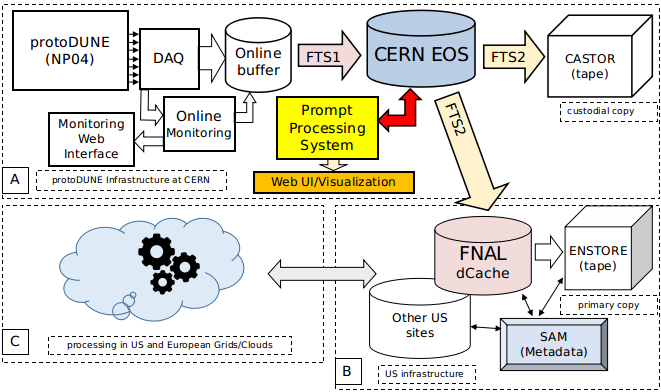
\includegraphics[width=0.9\textwidth]{figures/protoDUNE_data_flow_2018_v1.png}
\caption{\label{fig:dataflow}Diagram of the protoDUNE-SP data flow}
\end{figure}


\section{Data Quality Monitoring and Prompt Processing}
\subsection{DQM Applications}
The following types of applications were developed by the members of the DUNE Collaboration and
included in the \pd DQM suite during the detector
commissioning:
\begin{itemize}
\item Monitoring of front-end motherboards
\item LArTPC signal processing (noise reduction, deconvolution)
\item Basic event visualization in 2D
\item Initial data preparation for an advanced 3D event display running on a separate system
\item Liquid Argon purity monitoring using cosmic $\mu$ tracks
\item Estimation of the number of hits and charge collected in each section of the LArTPC, RMS of these values
\item Estimation of signal-to-noise ratio
\end{itemize}

\noindent For a few of these metrics the system produces time-series plots in addition to the tabulated data.
The DQM applications are often called \textit{payload jobs} so as to distinguish
them to service and infrastructure jobs which exist to support the function of the overall system.


\subsection{Design of the Prompt Processing System}

Computing resources for the Data Quality Monitoring in \pd-SP are managed by
the  \textit{\pd Prompt Processing System} (the ``p3s'')
which is separate from both the DAQ and the main production system. This is similar to some High-Energy Physics
experiments which implement ``express streams'' to perform preliminary calculations on the data very soon
after it leaves the DAQ.

The  p3s allows the experiment to benefit from combination of high capacity, high
performance distributed storage (CERN EOS), CERN networking resources and its Tier-0 computing facility.
By utilizing the pilot-based approach \cite{eps} to workload management which is the cornerstone of such well-known
systems as PanDA and DIRAC \cite{panda,dirac} p3s achieves low latency of automated job submission
as compared to running jobs directly on the batch trsource (which is currently HTCondor at CERN Tier-0).
In addition, since it combines a Web service and a back-end database this approach provides excellent
job monitoring capabilities.

% There are two pricipal components in the prompt processing system - a single instance
% of the p3s server and multiple pilots running on distributed resources.

%Pilot jobs (sometimes called \textit{agents}) as submitted to worker nodes which may be
%a part of a Grid site or a local batch system. Subsequently, each pilot sends a HTTP request to the p3s server
%to register and to try to obtain a description of a job that needs to be executed.
%Jobs descriptions exist as records in the p3s database as entries created independently from pilots by
%external clients (automatic or actuated by the user). The server matches a job records with a pilot and
%replies to its HTTP request with a message containing all necessary information needed for job
%execution (e.g. the path to the executable and the configuration file, additional environment variables etc).
%The pilot parses the message and initiates the job  execution. Once the job completes, the pilot repeats the cycle
%by sending anothe request to the server. The pilots are configured on the batch system to persist for a period
%of time much larger than typical execution time of the payload  jobs so the batch slot is already primed and the next
%job starts very quickly.

\subsection{Design of the DQM content service}
The results produced by the payload jobs managed by p3s can only be useful if there is an
efficient interface for the users to access these derived data. Such interface is provided in \pd-SP
by a Web service accessible through a Web browser and a few CLI utilities.
% Combination of
%functionality  p3s and DQM content servers in a single service is not the best solution since
%the workload management component (p3s) needs to maintain high availability and the extra
%load created by content requests has to be avoided.
The DQM output (the ``content'') can be stored in the system in two ways:
\begin{itemize}

\item When the basic unit of data that needs to be stored is a file e.g.\,an image in the PNG format such
file is stored on disk (EOS) and its location is recorded in a database so it can be later retrieved
and accessed through a dynamically generated Web page,  based on some selection criteria.
This is simplified by the fact that the EOS storage is directly accessible from the Apache server
used for this purpose.

\item When the basic unit of data is an array of numbers these are for the most part stored directly
in the database and are used in dynamically generated Web pages either in tabulated format or
to generate graphs by using Javascript.

\end{itemize}



\section{Technologies and Interfaces}
\subsection{Web Services}

Both p3s and the DQM content server ares implemented as Django \cite{django} applications
written in Python
with standard components such as the Apache Web server and PostgreSQL RDBMS as the backend storage
(a few other RDBMS can be used as well). All interactions with either service
are conducted via HTTP either from a Web browser or one of the included CLI utilities.
While the p3s instance deployed for \pd-SP is configured to use
the resources provided by CERN the system itself is platform-agnostic in the sense that it can manage
the resources of any cluster or group of worker nodes and in fact has been succesfully tested
in these scenarios as well.

The p3s server is responsible for workload management by matching available pilots to the job requests,
and also provides monitoring capabilities by allowing the user to browse and navigate
tabulated data describing the state of the various objects in the system (e.g. pilots, jobs, data files etc).
The design of the monitoring pages leverages the Django Web page template functionality and
the well known \textit{``django-tables2''} package which results
in a very small amout of application code. An example of pages served by p3s is
presented in Fig.\,\ref{fig:p3s_dash} (the p3s dashboard).

\begin{figure}[tb]
\centering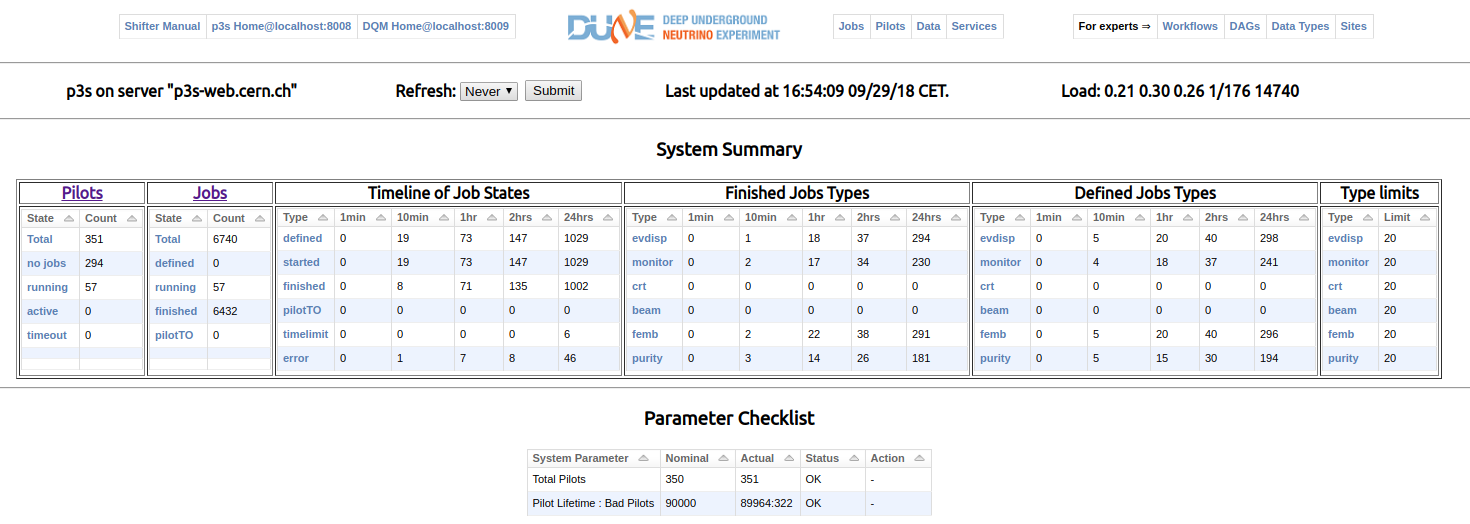
\includegraphics[width=1.0\textwidth]{figures/p3s_dash_2018_v1.png}
\caption{\label{fig:p3s_dash}The p3s dashboard}
\end{figure}

 A suite of CLI clients is provided as a component of p3s for managing pilots, jobs and
other entities. In case interaction with the server requires exhange of messages these are
formatted as JSON, pimarily because it is trivial to parse it in Python.

There is a centralized log of critical system messages stored in the p3s database which
is used to troubleshoot the system. It is also used to automatically generate alarms
for the operators should certain parameters fall out of their nominal range.

The p3s design also supports workflows described as Directed Acyclical Graphs (DAGs)
however in the current run of the experiment this functionality was not used.

\subsection{The Content Server Interface: the Self-Describing Data}
Due to highly dynamic nature of application development in the context of the \pd beam
test it is not practical to create static menus, links or make many assumptions about
the categories and content of plots and other data products coming out of the DQM.
Any such information or logic included in the server in a static manner would result
in frequent and time-consuming updates of the server code.

Instead, each DQM application is expected to produce two or more files in accordance
with simple JSON schemas. One file is referred to as ``summary'' and it contains basic
information about the attributes of the raw data file used as input, such the run number
and a few other indices. This file is stored as a JSON string in the back-end database
of the DQM server. It may also optionally contain a number of summary metrics
that are then parsed by the page-generating logic of the server and presented
in the DQM tables.

The second JSON file (or a group of files) referred to as ``description'' or ``file list'' provides references to
plots produced in formats such as PNG, as well as description of ``categories''
and sub-categories which are automatically translated by the server into
groups of menus with links necessary to access these plots on the dynamically generated
Web pages. An example of such menus is presented in Fig.\,\ref{fig:tpc_monitor}.
This approach greatly simplifies integration of different types of payload jobs 
and data into the DQM content service, with minimal or no changes to the
server code.

\begin{figure}[tb]
\centering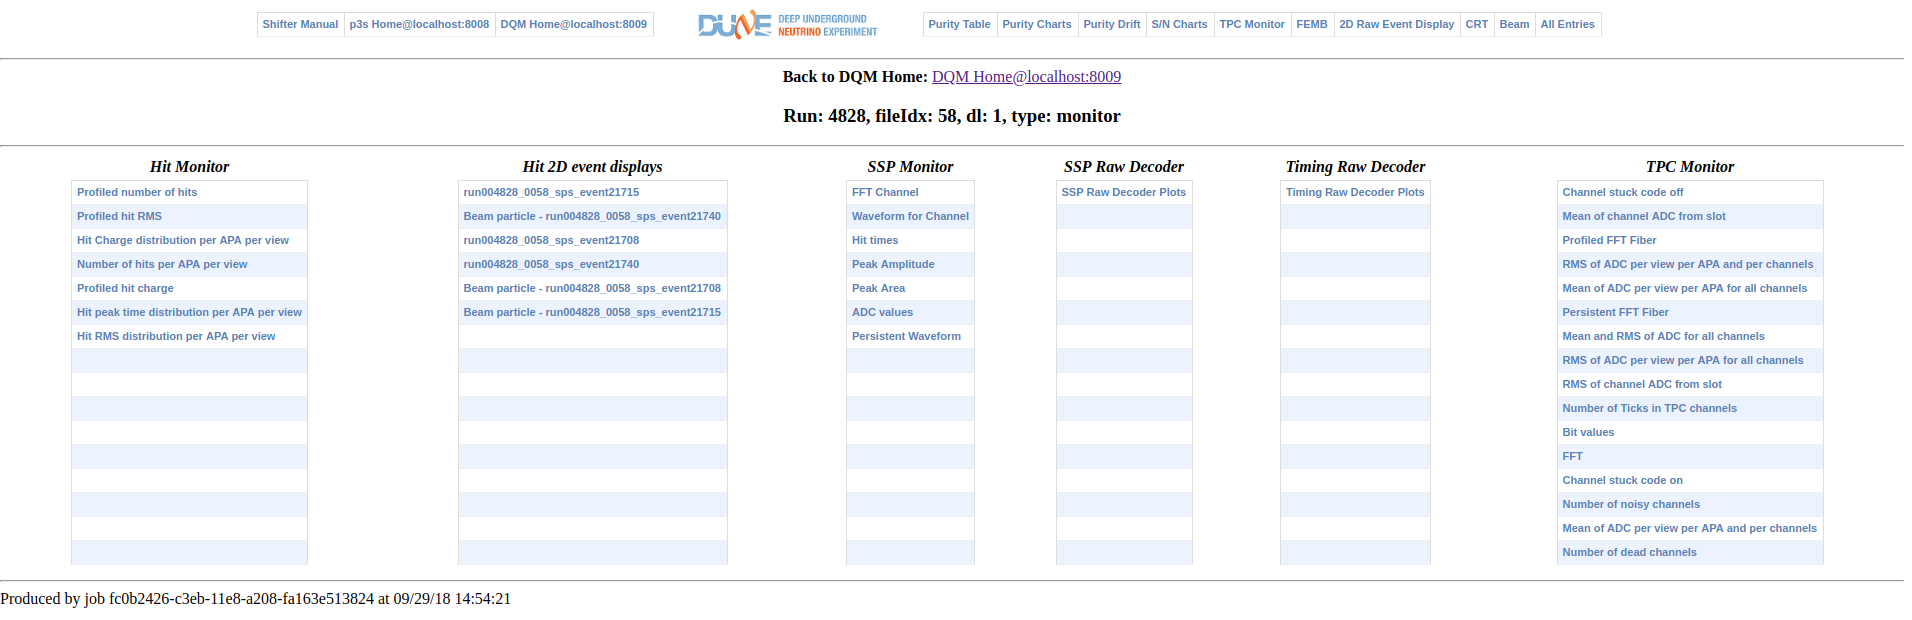
\includegraphics[width=1.0\textwidth]{figures/tpc_monitor_2018_v1.png}
\caption{\label{fig:tpc_monitor}An example of dynamically generated DQM menus and links}
\end{figure}


\begin{figure}[tb]
\centering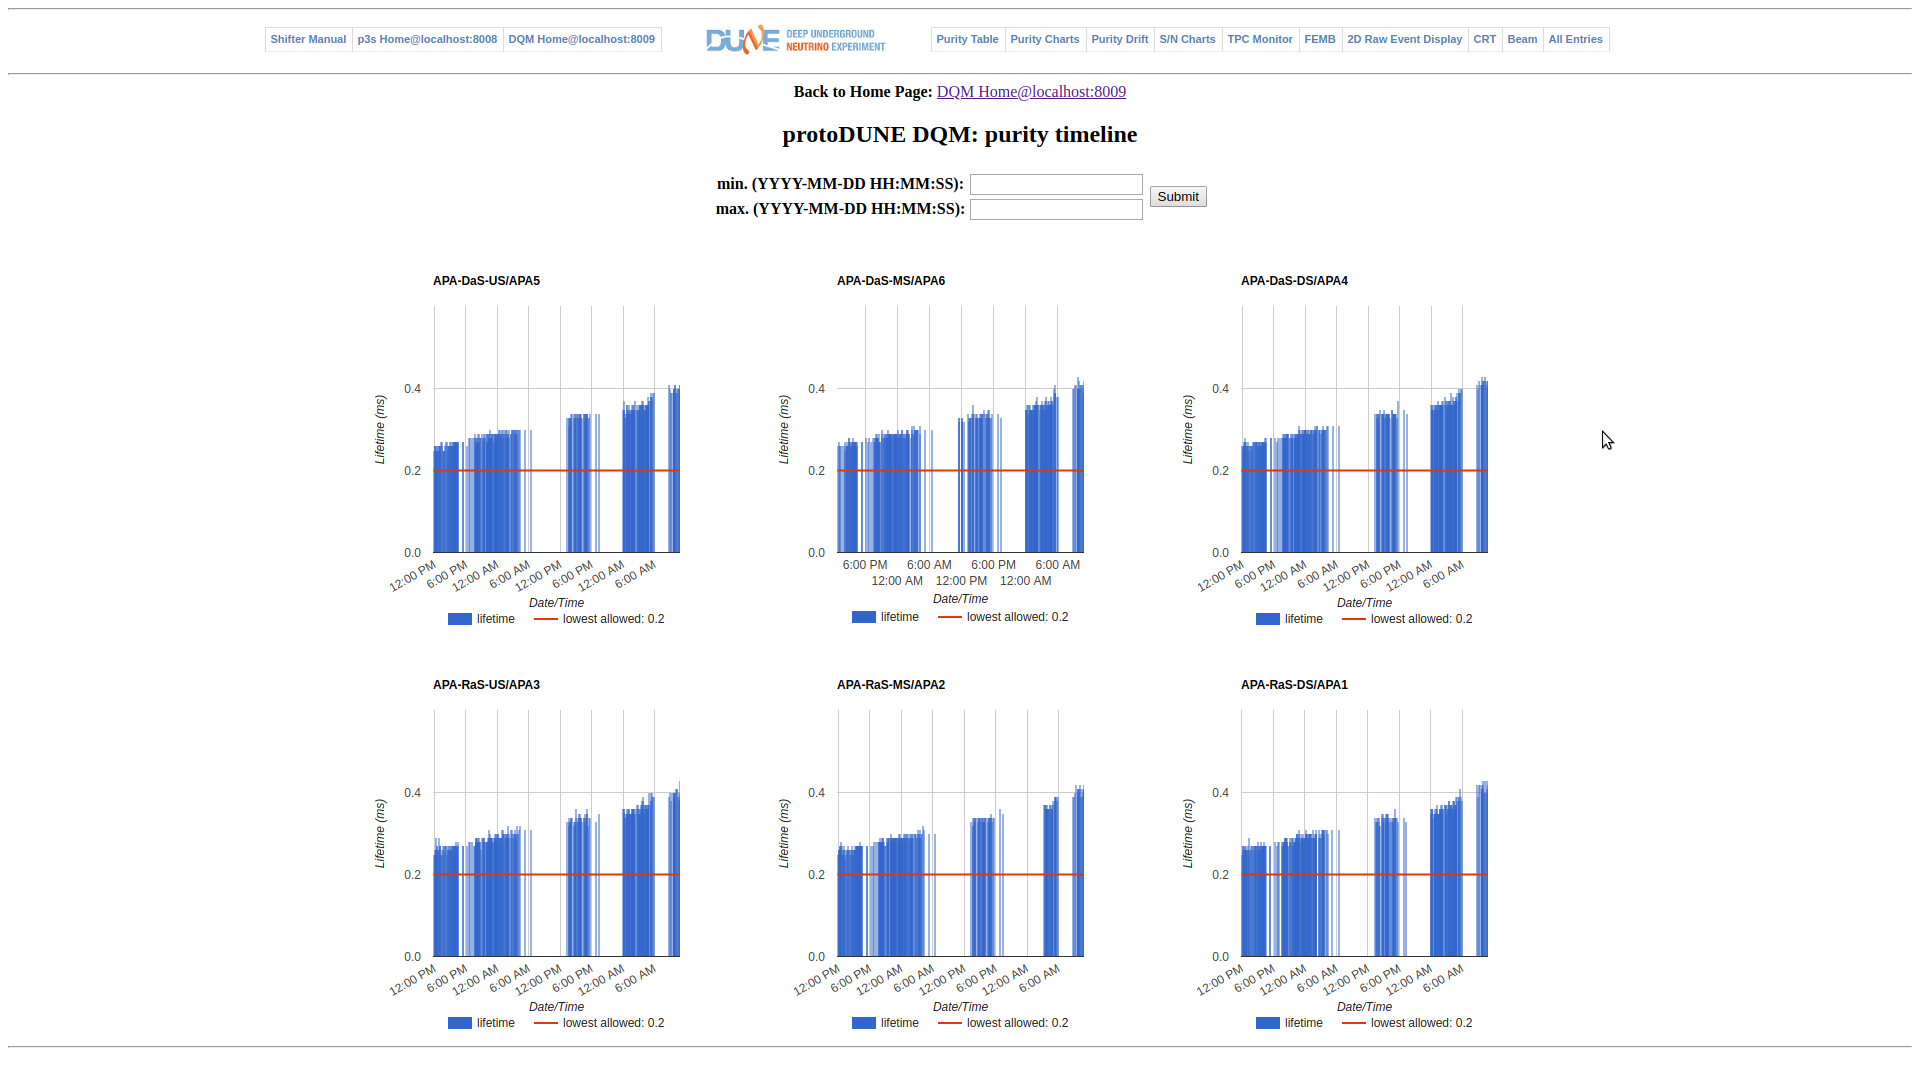
\includegraphics[width=1.0\textwidth]{figures/purity_chart_2018_v1.png}
\caption{\label{fig:purity_chart}An example of dynamically generated time series plot in DQM.}
\end{figure}

A few types of data in DQM can be accessed more efficiently if they are presented as time
series plots. To handle such cases a Web page template was created containing
Javascript code making use of Google Charts functionality, so that the time series
plots are generated on the fly at the time of the user's request, based on the content
of the DQM database.

\subsection{Deployment}

The code of p3s and the DQM content server is version-controlled using \textit{git}
and GitHub. Code updates are done by priviledged users by updating the code
on the servers from the repository and subsequent service restart.

The p3s and DQM services as well as their back-end database servers have been deployed on
virtual machines within the CERN OpenStack cloud. Processes that need to be run periodically,
i.e. refreshing the p3s pilot job population, automatic DQM job generation based on detection
of fresh raw data written to EOS etc are maintained using \textit{``acrontab''} which is a kerberized
distributed version of crontab used at the \textit{lxplus} interactive Linux facility CERN.

\section{Conclusions}

The \pd-SP experiment which started operation at CERN in 2018 requires adequate Data
Quality Monitoring. To meet these requirements the DUNE Collaboration has developed
and deployed Web services which manage the execution of the DQM jobs on the CERN
facilities and dynamic handling of the DQM data content with efficient user interfaces.
Emphasis was made on using existing and proven technologies such as Django
for the Web applicaiton framework, the concept of utilizing pilot jobs for
efficient workload distribution and a number of others. The \pd-SP prompt
processing and DQM software which it supports were successfully used during
the commissioning phase of the experiment and will remain an imporant part
of its ongoing operation.

%For tables use syntax in table~\ref{tab-1}.
%\begin{table}
%\centering
%\caption{Please write your table caption here}
%\label{tab-1}       % Give a unique label
% For LaTeX tables you can use
%\begin{tabular}{lll}
%\hline
%first & second & third  \\\hline
%number & number & number \\
%number & number & number \\\hline
%\end{tabular}
% Or use
%\vspace*{5cm}  % with the correct table height
%\end{table}
%
% BibTeX or Biber users please use (the style is already called in the class, ensure that the "woc.bst" style is in your local directory)
% \bibliography{name or your bibliography database}
%
% Non-BibTeX users please use
%


\begin{thebibliography}{99}



\bibitem{cdrVol1}
R. Acciarri et al.
\emph{Long-Baseline Neutrino Facility (LBNF) and Deep Underground Neutrino Experiment (DUNE) Conceptual Design Report Volume 1: The LBNF and DUNE Projects}.\\ ~e-Print: arXiv:\textbf{1601.05471}
 %DUNE CDR Vol 1 -- The LBNF and DUNE Projects.~e-Print: arXiv:1601.05471
%\url{http://arxiv.org/abs/1601.05471}

\bibitem{cdrVol4}
R. Acciarri et al.
\emph{Long-Baseline Neutrino Facility (LBNF) and Deep Underground Neutrino Experiment (DUNE) Conceptual Design Report, Volume 4: The DUNE Detectors at LBNF}.\\~e-Print: arXiv:\textbf{1601.02984}
%\url{http://arxiv.org/abs/1601.02984}

\bibitem{eps} M.Potekhin et al. \emph{The protoDUNE-SP experiment and its prompt
processing system}. Proceedings of Science (EPS-HEP2017) 513

%\bibitem{uboone}
%B. Jones et al.  \emph{The Status of the MicroBooNE Experiment.~J. Phys.: Conf. Series.} Vol.\textbf{408}. IOP Publishing, 2013,
%doi:10.1088/1742-6596/408/1/012028


\bibitem{sam}
R. A. Illingworth \emph{A data handling system for modern and future Fermilab experiments.~J. Phys.: Conf. Series.} Vol.\textbf{513}. IOP Publishing, 2014,
doi:10.1088/1742-6596/513/3/032045

\bibitem{fts}
A. Norman \emph{The Fermilab File Transfer System}.~e-Print: FNAL CD-DocDB-5412

\bibitem{castoreos}
 L. Mascetti et al. \emph{Disk storage at CERN.~J. Phys.: Conf. Series.} Vol.\textbf{664}. IOP Publishing, 2015,
doi:10.1088/1742-6596/664/4/042035

\bibitem{eos_role}
S. Fuess et al. \emph{Design of the protoDUNE raw data management
infrastructure.~J. Phys.: Conf. Series.} Vol.\textbf{898}. IOP Publishing, 2017,
doi:10.1088/1742-6596/898/6/062036

%\bibitem{xrootd}
%L. Bauerdick et al. \emph{Using Xrootd to Federate Regional Storage.~J. Phys.: Conf. Series.} Vol.\textbf{396}. IOP Publishing, 2012,
%doi:10.1088/1742-6596/396/4/042009

\bibitem{panda}
T. Maeno et al. \emph{Overview of ATLAS PanDA Workload Management.~J. Phys.: Conf. Series.} Vol.\textbf{331}. IOP Publishing, 2011,
doi:10.1088/1742-6596/331/7/072024



\bibitem{dirac}
A. Casajus et al.  \emph{DIRAC Pilot Framework and the DIRAC
Workload Management System.~J. Phys.: Conf. Series.} Vol.\textbf{219}. IOP Publishing, 2010,
doi:10.1088/1742-6596/219/6/062049

\bibitem{django}
N. George \emph{Mastering Django: Core. The Complete Guide to Django 1.8 LTS}~ GNW Independent Publishing, ISBN: 099461683X



\end{thebibliography}


\end{document}

% end of file template.tex

%\begin{table}
%\begin{center}
%\caption{\label{table:np04_data_rate}
% protoDUNE-SP readout parameters}
%\ \\
%\begin{tabularx}{0.75\textwidth}{ X  >{\setlength{\hsize}{0.8\hsize}}r}
%\hline
%Detector Parameter & Target \\
%\hline
%TPC channel count & 15,360 \\
%Digitization frequency & 2\,MHz \\
%Nominal electron drift time & 2.2\,ms\\
%Nominal electron drift velocity & 1.6\,mm/$\mu$s\\
%Readout window & 5\,ms \\
%SPS spill time& 4.8\,s\\
%SPS cycle& 22.5\,s\\
%Nominal trigger rate & 25\,Hz \\
%Single readout size (per trigger) & 230.4\,MB \\
%Lossless compression factor (estimated) & 4 \\
%Instantaneous data rate (in-spill) & 1440\,MB/s \\
%Average data rate & 300\,MB/s \\
%Total data recorded (beam + cosmic) & 3\,PB\\
%Buffer to store 3 days worth of data & 300\,TB\\
%\hline
%\end{tabularx}
%\end{center}
%\end{table}

